
\subsection{コマンドの命名原則}
機能ごとの動作はコマンドのオプションによって指定されます.
このオプションにどのような名前をつけるかは,どれだけコマンドを覚えやすいかという
意味で重要です.コマンドの振る舞いを的確に表す名称をつける必要があります.

この振る舞いとしてもっとも受け入れやすいのがshellで用意されているコマンドです.
pwd, ls, rm, touch, openなどはもっとも直感的に動作がわかるコマンドです.
hikiutilsの振る舞いを予測できるシェルコマンドと同じ名前でオプションを提供する
ようにします.

\subsubsection{hikiutilsの想定利用形態}
ここでhikiutilsがあらかじめ想定している利用形態を解説しておきます.
\begin{quote}\begin{verbatim}
!!!caption:hikiutilsがあらかじめ想定している利用形態.
=======
!!!caption:(fig:002)hikiutilsがあらかじめ想定している利用形態.
\end{verbatim}\end{quote}
\begin{figure}[htbp]\begin{center}
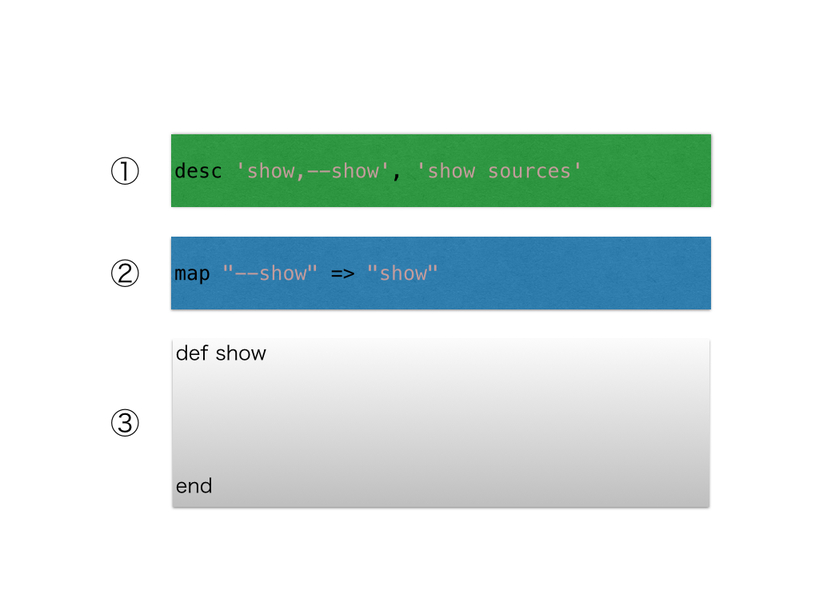
\includegraphics[width=10cm,bb= 0 0 737 553]{../figs/./hikiutils_yamane.002.jpg}
\caption{}
\label{default}\end{center}\end{figure}
hikiutilsは,

\begin{itemize}
\item local PCとglobal serverとが用意されており,
\item それらのデータをrsyncで同期する
\end{itemize}
ことで動作することを想定しています.これは,ネットに繋がっていないオフラインの状況でも
テキストなどの編集が可能で,さらに不用意な書き換えを防ぐための機構です.さらに,
どちらもが何かあった時のバックアップともなって,ミスによる手戻りを防いでいます.

これらの設定は,~/.hikircにyaml形式で記述・保存されています.
\begin{lstlisting}[style=]
bob% cat ~/.hikirc
:srcs:
- :nick_name: new_ist
  :local_dir: "/Users/bob/Sites/new_ist_data/ist_data"
  :local_uri: http://localhost/ist
  :global_dir: nishitani@ist.ksc.kwansei.ac.jp:/home/nishitani/new_ist_data/ist_data
  :global_uri: http://ist.ksc.kwansei.ac.jp/~nishitani/
- :nick_name: dmz0
  :local_dir: "/Users/bob/Sites/nishitani0/Internal/data"
  :local_uri: http://localhost/~bob/nishitani0/Internal
  :global_dir: bob@dmz0:/Users/bob/Sites/nishitani0/Internal/data
  :global_uri: http://nishitani0.kwansei.ac.jp/~bob/nishitani0/Internal
\end{lstlisting}
また,一般的に一人のユーザがいくつものまとまりとしてのlocal-globalペアを
保持して管理することが普通です.それぞれにnicke\_nameをつけて管理しています.
\begin{lstlisting}[style=]
bob% hiki -s
hikiutils: provide utilities for helping hiki editing.
"open -a mi"
target_no:1
editor_command:open -a mi
 id | name      | local directory                           | global uri     
-----------------------------------------------------------------------------
  0 | new_ist   | /Users/bob/Sites/new_ist_data/ist_data    | http://ist.ksc.k
 *1 | dmz0      | /Users/bob/Sites/nishitani0/Internal/data | http://nishitani
  2 | ist       | /Users/bob/Sites/hiki-data/data           | http://ist.ksc.k
  3 | new_maple | /Users/bob/Sites/new_ist_data/maple_hiki_d| http://ist.ksc.k
\end{lstlisting}
とすると,それらの一覧と,いまtargetにしているnick\_nameディレクリが表示されます.

\subsubsection{コメンド名と振る舞いの詳細}
検討の結果コマンドを以下のように書き換えることとします.
上部に記した,特によく使うコマンドに関しては,shellでよく使われるコマンド名と一致するにようにしました.

\begin{table}[htbp]\begin{center}
\caption{}
\begin{tabular}{llll}
\hline
変更前  &変更後  &動作の解説  \\ \hline
edit FILE         &open  &open file  \\
list [FILE]       &ls  &list files  \\
rsync             &rsync  &rsync files  \\
update FILE       &touch  &update file  \\
show              &pwd  &show nick\_names  \\
target VAL        &cd  &targetを変える,cdとのメタファ  \\
  &  \\
move [FILE]       &mv  &move file  \\
remove [FILE]     &rm  &remove files  \\
add               &  &add sources info  \\
checkdb           &  &check database file  \\
datebase FILE     &db  &read datebase file  \\
display FILE      &show  &display converted hikifile  \\
euc FILE          &  &translate file to euc  \\
help [COMMAND]    &-h  &Describe available commands  \\
version           &-v  &show program version  \\
\hline
\end{tabular}
\label{default}
\end{center}\end{table}
%for inserting separate lines, use \hline, \cline{2-3} etc.

それぞれの意図を動作の解説として記述しています.

\paragraph{open FILE}
ファイルを編集のためにeditorでopen.Editorは~/.hikircに
\begin{quote}\begin{verbatim}
:editor_command: open -a mi
\end{verbatim}\end{quote}
として保存されている.open -a miをemacsなどに適宜変更して使用.

\paragraph{ls [FILE]}
local\_dirにあるファイル名を[FILE*]として表示.例えば,hikiutils\_yamane以下の拡張子が
ついたファイルを表示.hikiシステムではtextディレクトリーは階層構造を取ることができない.
西谷研ではdirectoryの代わりにスネーク表記で階層構造を表している.

\paragraph{rsync}
local\_dirの内容をglobal\_dirにrsyncする.逆方向は同期に誤差が生じたり,permissionが
おかしくなるので,現在のところ一方向の同期のみとしている.したがって,作業手順としては
テキストの変更はlocal\_dirで読み行うようにしている.

\paragraph{touch FILE}
loccal\_dirで書き換えたFILEの内容をlocal\_uriに反映させ,ブラウザで表示.シェルコマンドの
touchによって,変更時間を現在に変え,最新状態とするのに似せてコマンド名をtouchとしている.

\paragraph{pwd}
nick\_nameの一覧とtargetを表示,current targetをcurrent dirとみなして,
コマンド名をpwdとした.

\paragraph{cd VAL}
targetを変える,change directoryとのメタファ.ただし,いまのところnick\_nameでは
対応しておらず,nick\_nameの番号をVAL入力することで変更する.

